\chap{3D旋转变换}
\section{介绍}
在本章中,我们回顾了在计算机图形软件中使用的三维欧拉旋转变换。特别地,我们确定了他们的阿喀琉斯之踵——万向节锁——以及能够围绕任意轴旋转的需求。为此,我们将开发一个实现这种旋转的矩阵变换,并在下一章中使用四元数开发一个类似的变换。

\section{3D旋转变换}
旋转点和参考系的传统技术是基于欧拉旋转,以瑞士数学家Leonhard Euler的名字命名。他们提供了三种轮换的方法。第一种是绕三个笛卡尔轴之一旋转。第二个组合了任意两个围绕不同轴的旋转,第三个组合了任意三个旋转。

最初,这种方法听起来很吸引人——在许多情况下效果很好,然而,这种技术存在一些问题。第一个问题是,当两个或多个旋转结合在一起时,很难可视化和预测最终的旋转将如何表现。第二点是,绕一个特定的轴旋转是很复杂的,第三点是,在某些条件下,人们失去了对物体的一个旋转轴的访问。最后一个问题被称为万向节锁。为了理解这些问题,我们将构建一个受万向节锁定影响的三维旋转变换。

\section{绕笛卡尔轴旋转}
一个点在平面上绕原点旋转的变换由
$$
\mathbf{R}_{\beta}=\left[\begin{array}{cc}
\cos \beta & -\sin \beta \\
\sin \beta & \cos \beta
\end{array}\right] .
$$

这可以通过添加第三个坐标推广到围绕笛卡尔轴的三维旋转。例如,要绕$z$-轴旋转,我们添加一个$z$-坐标,如下所示:
$$
\mathbf{R}_{\beta, z}=\left[\begin{array}{ccc}
\cos \beta & -\sin \beta & 0 \\
\sin \beta & \cos \beta & 0 \\
0 & 0 & 1
\end{array}\right]
$$

\begin{figure}[h!]
    \centering
    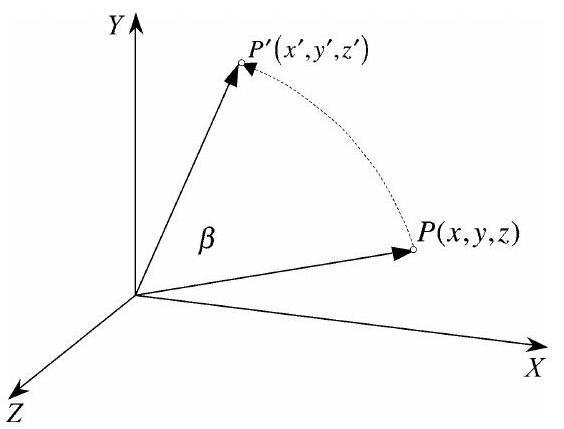
\includegraphics[max width=0.5\textwidth]{2023_01_16_a848224efad29cd66460g-089}
    \caption[short]{点 $P$ 围绕 $z$ 轴旋转}
\end{figure}

如图6.1所示。要围绕$x$-轴旋转一个点,$x$-坐标保持不变,而$y$ -和$z$-坐标根据$2 \mathrm{D}$旋转变换进行更改:
$$
\mathbf{R}_{\beta, x}=\left[\begin{array}{ccc}
1 & 0 & 0 \\
0 & \cos \beta & -\sin \beta \\
0 & \sin \beta & \cos \beta
\end{array}\right] .
$$

最后,为了绕$y$-轴旋转,$y$-坐标保持不变,而$x$和$z$-坐标改变:
$$
\mathbf{R}_{\beta, y}=\left[\begin{array}{ccc}
\cos \beta & 0 & \sin \beta \\
0 & 1 & 0 \\
-\sin \beta & 0 & \cos \beta
\end{array}\right] .
$$

\section{绕偏移轴旋转}
要绕与笛卡尔轴之一平行的轴旋转,通常采用齐次坐标并平移要旋转的点,这样它可以绕原点旋转,然后平移回来一个相等且相反的量。假定读者熟悉这种策略。但是,为了完整起见,我们将构造一个变换,使一个点围绕一个与$z$-轴平行的轴旋转,并与点$\left(t_{x}, t_{y}, 0\right)$相交,如图6.2所示:
$$
\left[\begin{array}{c}
x^{\prime} \\
y^{\prime} \\
z^{\prime} \\
1
\end{array}\right]=\mathbf{T}_{t_{x}, t_{y}, 0} \mathbf{R}_{\beta, z} \mathbf{T}_{-t_{x},-t_{y}, 0}\left[\begin{array}{c}
x \\
y \\
z \\
1
\end{array}\right]
$$

\begin{figure}
    \centering
    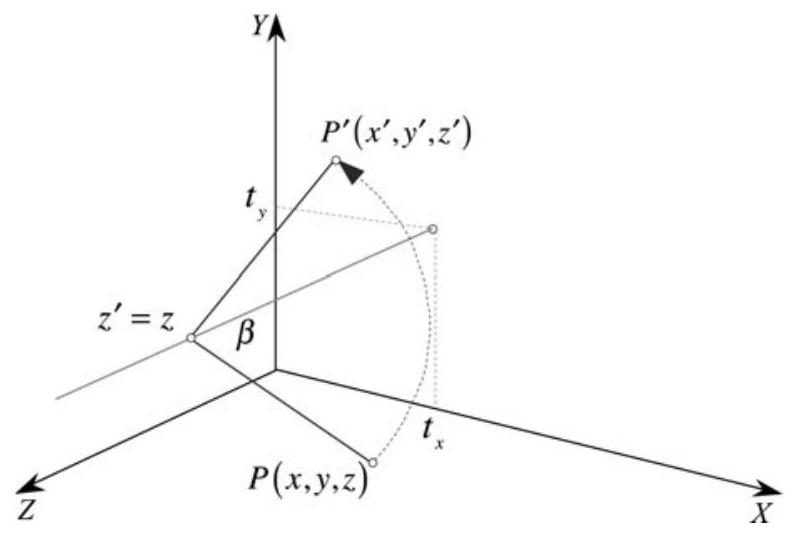
\includegraphics[max width=0.6\textwidth]{2023_01_16_a848224efad29cd66460g-090}
    \caption[short]{绕平行于$z$-轴的轴旋转一点}
\end{figure}

其中
$$
\begin{aligned}
& \mathbf{T}_{-t_{x},-t_{y}, 0} && \text { 创建临时原点 } \\
& \mathbf{R}_{\beta, z} && \text { 围绕临时的 } z \text {轴旋转 }\beta \text{角度} \\
& \mathbf{T}_{t_{x}, t_{y}, 0} && \text { 回到原来的坐标系中的位置 }
\end{aligned}
$$

矩阵变换是
$$
\mathbf{R}_{\beta, z,\left(t_{x}, t_{y}, 0\right)}=\left[\begin{array}{cccc}
\cos \beta & -\sin \beta & 0 & t_{x}(1-\cos \beta)+t_{y} \sin \beta \\
\sin \beta & \cos \beta & 0 & t_{y}(1-\cos \beta)-t_{x} \sin \beta \\
0 & 0 & 1 & 0 \\
0 & 0 & 0 & 1
\end{array}\right]
$$

围绕平行于$x$-轴和平行于$y$-轴的偏移轴旋转的矩阵为:
$$
\begin{aligned}
\mathbf{R}_{\beta, x,\left(0, t_{y}, t_{z}\right)} & =\left[\begin{array}{cccc}
1 & 0 & 0 & 0 \\
0 & \cos \beta & -\sin \beta & t_{y}(1-\cos \beta)+t_{z} \sin \beta \\
0 & \sin \beta & \cos \beta & t_{z}(1-\cos \beta)-t_{y} \sin \beta \\
0 & 0 & 0 & 1
\end{array}\right] \\
\mathbf{R}_{\beta, y,\left(t_{x}, 0, t_{z}\right)} & =\left[\begin{array}{cccc}
\cos \beta & 0 & \sin \beta & t_{x}(1-\cos \beta)-t_{z} \sin \beta \\
0 & 1 & 0 & 0 \\
-\sin \beta & 0 & \cos \beta & t_{z}(1-\cos \beta)+t_{x} \sin \beta \\
0 & 0 & 0 & 1
\end{array}\right] .
\end{aligned}
$$

\section{复合旋转}
撇开围绕单轴和偏移轴旋转的变换不谈,我们有三个围绕笛卡尔轴旋转的变换:$\mathbf{R}_{\alpha, x}, \mathbf{R}_{\beta, y}$和$\mathbf{R}_{\gamma, z}$,它们可以组合成双变换族和三重变换族。如上所述,这种旋转称为欧拉旋转,假定读者熟悉其结构。三重变换族是:
$$
\begin{array}{llll}
\mathbf{R}_{\gamma, x} \mathbf{R}_{\beta, y} \mathbf{R}_{\alpha, x} & \mathbf{R}_{\gamma, x} \mathbf{R}_{\beta, y} \mathbf{R}_{\alpha, z} & \mathbf{R}_{\gamma, x} \mathbf{R}_{\beta, z} \mathbf{R}_{\alpha, x} & \mathbf{R}_{\gamma, x} \mathbf{R}_{\beta, z} \mathbf{R}_{\alpha, y} \\
\mathbf{R}_{\gamma, y} \mathbf{R}_{\beta, x} \mathbf{R}_{\alpha, y} & \mathbf{R}_{\gamma, y} \mathbf{R}_{\beta, x} \mathbf{R}_{\alpha, z} & \mathbf{R}_{\gamma, y} \mathbf{R}_{\beta, z} \mathbf{R}_{\alpha, x} & \mathbf{R}_{\gamma, y} \mathbf{R}_{\beta, z} \mathbf{R}_{\alpha, y} \\
\mathbf{R}_{\gamma, z} \mathbf{R}_{\beta, x} \mathbf{R}_{\alpha, y} & \mathbf{R}_{\gamma, z} \mathbf{R}_{\beta, x} \mathbf{R}_{\alpha, z} & \mathbf{R}_{\gamma, z} \mathbf{R}_{\beta, y} \mathbf{R}_{\alpha, x} & \mathbf{R}_{\gamma, z} \mathbf{R}_{\beta, y} \mathbf{R}_{\alpha, z} .
\end{array}
$$

为了说明万向节锁的问题,我们将使用一个立方体,其顶点编号为0到7,如图6.3所示。
\begin{figure}[h!]
    \centering
    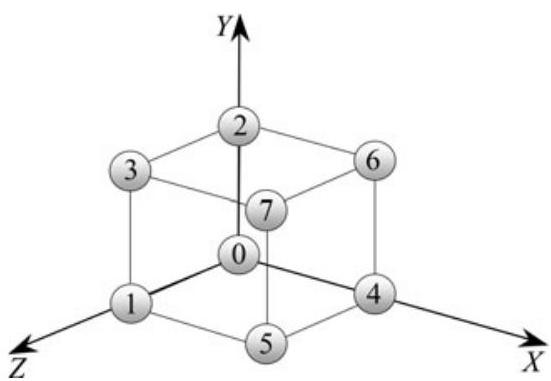
\includegraphics[max width=0.4\textwidth]{2023_01_16_a848224efad29cd66460g-091}
    \caption[short]{位于原点的单位立方体}
\end{figure}

\begin{figure}[h!]
    \centering
    \subfigure[]{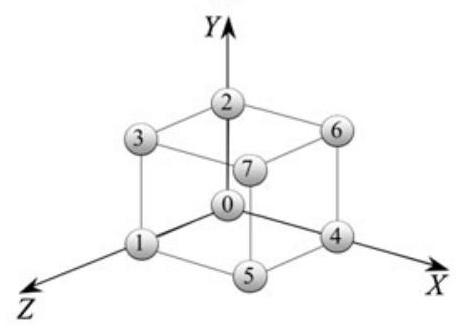
\includegraphics[max width=0.35\textwidth]{2023_01_16_a848224efad29cd66460g-091(1)}}
    \subfigure[]{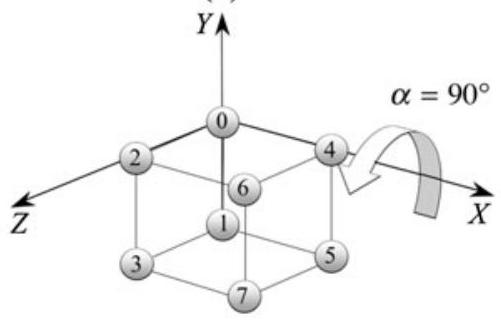
\includegraphics[max width=0.35\textwidth]{2023_01_16_a848224efad29cd66460g-091(3)}}\\
    \subfigure[]{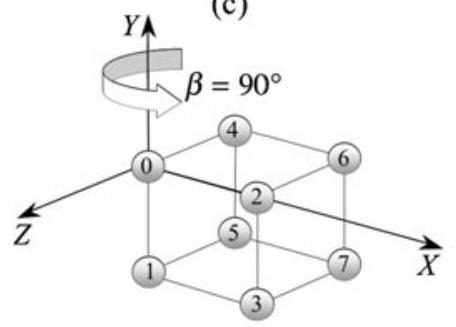
\includegraphics[max width=0.35\textwidth]{2023_01_16_a848224efad29cd66460g-091(2)}}
    \subfigure[]{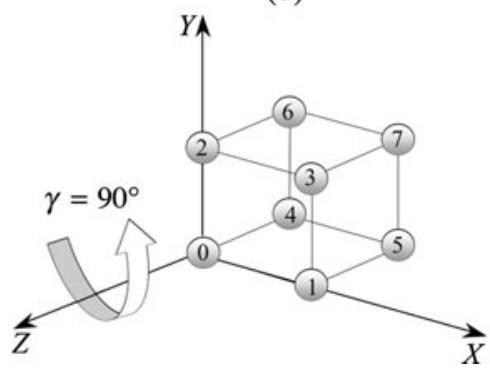
\includegraphics[max width=0.35\textwidth]{2023_01_16_a848224efad29cd66460g-091(4)}}
    \caption[short]{单位立方体在三次旋转之前和期间的四个视图}
\end{figure}

我们可以通过在任意序列中放置$\mathbf{R}_{\alpha, x}, \mathbf{R}_{\beta, y}$和$\mathbf{R}_{\gamma, z}$来创建复合旋转变换——甚至可以重复其中一个序列两次,只要它们被不同的变换隔开。作为后者的一个例子,我们可以使用序列$\mathbf{R}_{\alpha, z} \mathbf{R}_{\beta, y} \mathbf{R}_{\gamma, z}$,其中我们围绕$z$-轴旋转两次。然而,为了说明万向节锁,让我们选择序列$\mathbf{R}_{\gamma, z} \mathbf{R}_{\beta, y} \mathbf{R}_{\alpha, x}$,并使$\alpha=\beta=\gamma=90^{\circ}$,这相当于围绕固定的$x$-轴旋转一个点$90^{\circ}$,然后围绕固定的$y$-轴旋转$90^{\circ}$,然后围绕固定的$z$-轴旋转$90^{\circ}$。该旋转序列如图6.4所示。

\begin{figure}[h!]
    \centering
    \subfigure[]{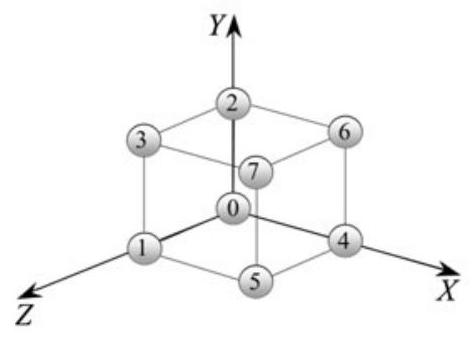
\includegraphics[max width=0.35\textwidth]{2023_01_16_a848224efad29cd66460g-092}}
    \subfigure[]{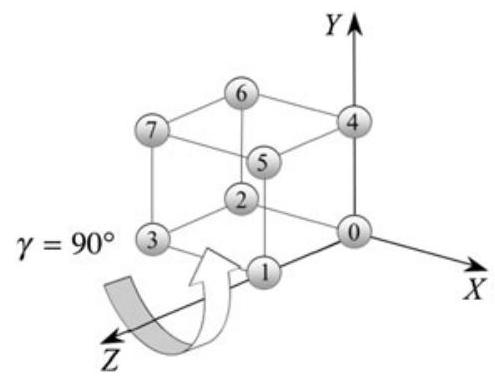
\includegraphics[max width=0.35\textwidth]{2023_01_16_a848224efad29cd66460g-092(2)}}\\
    \subfigure[]{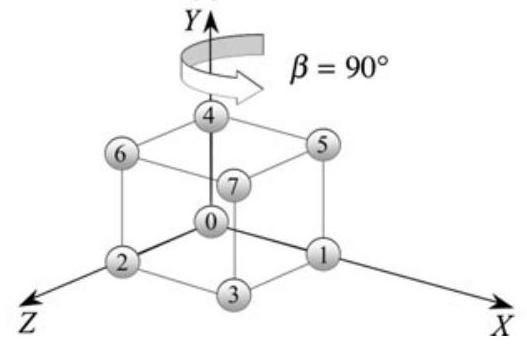
\includegraphics[max width=0.35\textwidth]{2023_01_16_a848224efad29cd66460g-092(1)}}
    \subfigure[]{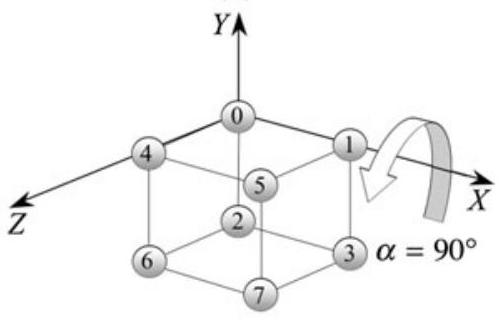
\includegraphics[max width=0.35\textwidth]{2023_01_16_a848224efad29cd66460g-092(3)}}
    \caption[short]{使用旋转序列$\mathbf{R}_{\alpha, x} \mathbf{R}_{\beta, y} \mathbf{R}_{\gamma, z}$的单位立方体的四个视图}
\end{figure}

图$6.4$ (a)显示了立方体的起始位置;(b)在绕$x$轴旋转$90^{\circ}$后显示其位置;(c)在绕$y$轴进一步旋转$90^{\circ}$后显示其位置;(d)立方体绕z轴旋转$90^{\circ}$后的静止位置。

然而,尽管采用了围绕不同轴的三次旋转,立方体实际上只围绕$y$轴旋转了$90^{\circ}$!立方体绕着穿过顶点0和4的轴旋转了两次,绕着穿过顶点0和1的轴旋转了一次,但是穿过顶点0和2的轴被忽略了。这被称为万向节锁定,并通过一个不幸的旋转序列组合和角度而产生。

将复合旋转反转到$\mathbf{R}_{\alpha, x} \mathbf{R}_{\beta, y} \mathbf{R}_{\gamma, z}$并不能改善问题。这个复合变换等价于围绕固定的z轴旋转一个点$90^{\circ}$,然后围绕固定的$y$-轴旋转$90^{\circ}$,然后围绕固定的$x$-轴旋转$90^{\circ}$。该旋转序列如图6.5所示。

对图$6.5$ (d)的检查显示,单位立方体已经围绕向量$\left[\begin{array}{lll}1 & 0 & 1\end{array}\right]^{\mathrm{T}}$旋转了$180^{\circ}$,即一个与顶点0和5相交的轴。这一次,立方体围绕与顶点0和1相交的轴旋转了两次,围绕与顶点0和4相交的轴旋转了一次,同样,与顶点0和2相交的轴被忽略了。不难看出为什么欧拉旋转会引起这么多问题。让我们继续,看看如何绕任意轴旋转。



\section{绕任意轴旋转}
单个欧拉变换并没有本质上的问题,问题是它们组合在一起产生旋转的方式有缺陷。理想情况下,我们需要一个旋转变换,允许我们指定轴和旋转角度,这是我们要计算的。第一种方法使用矩阵和三角函数,相当费力。第二种方法采用矢量分析,非常简洁。

\subsection{矩阵}
我们首先使用单位向量$\hat{\mathbf{n}}$定义一个轴,其中一个点$P$被旋转到$P^{\prime}$,如图6.6所示。由于我们只能使用围绕笛卡尔轴旋转点的矩阵,所以这个单位向量必须暂时与笛卡尔轴对齐。在下面的例子中,我们选择$x$-轴。在对齐过程中,点$P$进行必要的转换,以使单位向量与$x$-轴对齐。然后我们绕$x$轴旋转$P$。为了完成该操作,旋转后的点进行变换,使单位向量返回到其原始坐标系位置。

\begin{figure}[h!]
    \centering
    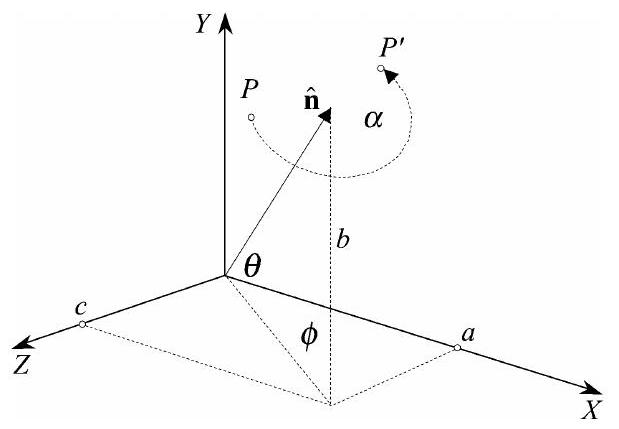
\includegraphics[max width=0.5\textwidth]{2023_01_16_a848224efad29cd66460g-093}
    \caption[short]{绕任意轴旋转的几何图形}
\end{figure}

虽然矩阵为这类工作提供了强大的工具,但它非常乏味,但却是提高一个人代数技能的好练习!

图$6.6$显示了一个点$P(x, y, z)$围绕如下定义的轴旋转一个角度$\alpha$到$\alpha$ to $P^{\prime}\left(x^{\prime}, y^{\prime}, z^{\prime}\right)$ 
$$
\hat{\mathbf{n}}=a \mathbf{i}+b \mathbf{j}+c \mathbf{k} .
$$

实现该操作的转换表达式如下:
$$
\left[\begin{array}{c}
x^{\prime} \\
y^{\prime} \\
z^{\prime}
\end{array}\right]=\mathbf{R}_{-\phi, y} \mathbf{R}_{\theta, z} \mathbf{R}_{\alpha, x} \mathbf{R}_{-\theta, z} \mathbf{R}_{\phi, y}\left[\begin{array}{c}
x \\
y \\
z
\end{array}\right]
$$

它将旋转轴与$x$-轴对齐,执行$P$的旋转,通过一个角度$\alpha$关于$x$-轴,并将旋转轴返回到其原始坐标系位置。因此,

$$
\begin{aligned}
\mathbf{R}_{\phi, y}= & {\left[\begin{array}{ccc}
\cos \phi & 0 & \sin \phi \\
0 & 1 & 0 \\
-\sin \phi & 0 & \cos \phi
\end{array}\right] } \\
\mathbf{R}_{\alpha, x}= & {\left[\begin{array}{ccc}
1 & 0 & 0 \\
0 & \cos \alpha & -\sin \alpha \\
0 & \sin \alpha & \cos \alpha
\end{array}\right] \mathbf{R}_{-\theta, z}=\left[\begin{array}{ccc}
\cos \theta & \sin \theta & 0 \\
-\sin \theta & \cos \theta & 0 \\
0 & 0 & 1
\end{array}\right] } \\
\mathbf{R}_{-\phi, y}= & {\left[\begin{array}{ccc}
\cos \phi & 0 & -\sin \phi \\
0 & 1 & 0 \\
\sin \phi & 0 & \cos \phi
\end{array}\right] }
\end{aligned}
$$

令
$$
\mathbf{R}_{-\phi, y} \mathbf{R}_{\theta, z} \mathbf{R}_{\alpha, x} \mathbf{R}_{-\theta, z} \mathbf{R}_{\phi, y}=\left[\begin{array}{lll}
a_{11} & a_{12} & a_{13} \\
a_{21} & a_{22} & a_{23} \\
a_{31} & a_{32} & a_{33}
\end{array}\right]
$$

其中,通过将矩阵相乘,我们发现:
$$
\begin{aligned}
a_{11}= & \cos ^{2} \phi \cos ^{2} \theta+\cos ^{2} \phi \sin ^{2} \theta \cos \alpha+\sin ^{2} \phi \cos \alpha \\
a_{12}= & \cos \phi \cos \theta \sin \theta-\cos \phi \sin \theta \cos \theta \cos \alpha-\sin \phi \cos \theta \sin \alpha \\
a_{13}= & \cos \phi \sin \phi \cos ^{2} \theta+\cos \phi \sin \phi \sin ^{2} \theta \cos \alpha+\sin ^{2} \phi \sin \theta \sin \alpha \\
& +\cos ^{2} \phi \sin \theta \sin \alpha-\cos \phi \sin \phi \cos \alpha \\
a_{21}= & \sin \theta \cos \theta \cos \phi-\cos \theta \sin \theta \cos \phi \cos \alpha+\cos \theta \sin \phi \sin \alpha \\
a_{22}= & \sin ^{2} \theta+\cos ^{2} \theta \cos \alpha \\
a_{23}= & \sin \theta \cos \theta \sin \phi-\cos \theta \sin \theta \sin \phi \cos \alpha-\cos \theta \cos \phi \sin \alpha \\
a_{31}= & \cos \phi \sin \phi \cos ^{2} \theta+\cos \phi \sin \phi \sin ^{2} \theta \cos \alpha-\cos 2 \phi \sin \theta \sin \alpha \\
= & -\cos \phi \sin \phi \cos \alpha \\
a_{32}= & \sin \phi \cos \theta \sin \theta-\sin \phi \sin ^{2} \theta \cos ^{2} \theta \cos \alpha+\cos \phi \cos \theta \sin \alpha \\
a_{33}= & \sin ^{2} \phi \cos \theta+\sin ^{2} \phi \sin ^{2} \theta \cos ^{2} \alpha-\cos \phi \sin \phi \sin \theta \sin \alpha \\
& +\cos \phi \sin \phi \sin \theta \sin \alpha+\cos ^{2} \phi \cos \alpha .
\end{aligned}
$$

经过大量的三角替换,我们得到了变换
$$
\left[\begin{array}{c}
x_{p}^{\prime} \\
y_{p}^{\prime} \\
z_{p}^{\prime}
\end{array}\right]=\left[\begin{array}{ccc}
a^{2} K+\cos \alpha & a b K-c \sin \alpha & a c K+b \sin \alpha \\
a b K+c \sin \alpha & b^{2} K+\cos \alpha & b c K-a \sin \alpha \\
a c K-b \sin \alpha & b c K+a \sin \alpha & c^{2} K+\cos \alpha
\end{array}\right]\left[\begin{array}{l}
x_{p} \\
y_{p} \\
z_{p}
\end{array}\right]
$$

其中
$$
K=1-\cos \alpha .
$$






\subsection{向量}
现在我们用向量来解决同样的问题。图$6.7$显示了与手头任务相关的几何视图。为了说明,图6.8显示了几何图形的横截面和平面图。

旋转轴由单位向量给出
$$
\hat{\mathbf{n}}=a \mathbf{i}+b \mathbf{j}+c \mathbf{k} .
$$
$P\left(x_{p}, y_{p}, z_{p}\right)$是将旋转$\alpha$角度到$P^{\prime}\left(x_{P}^{\prime}, y_{P}^{\prime}, z_{P}^{\prime}\right)$的点。

$O$是原点,$\mathbf{p}$和$\mathbf{p}^{\prime}$分别是$ P $和$ P ^{\prime}$的位置向量。
\begin{figure}[h!]
    \centering
    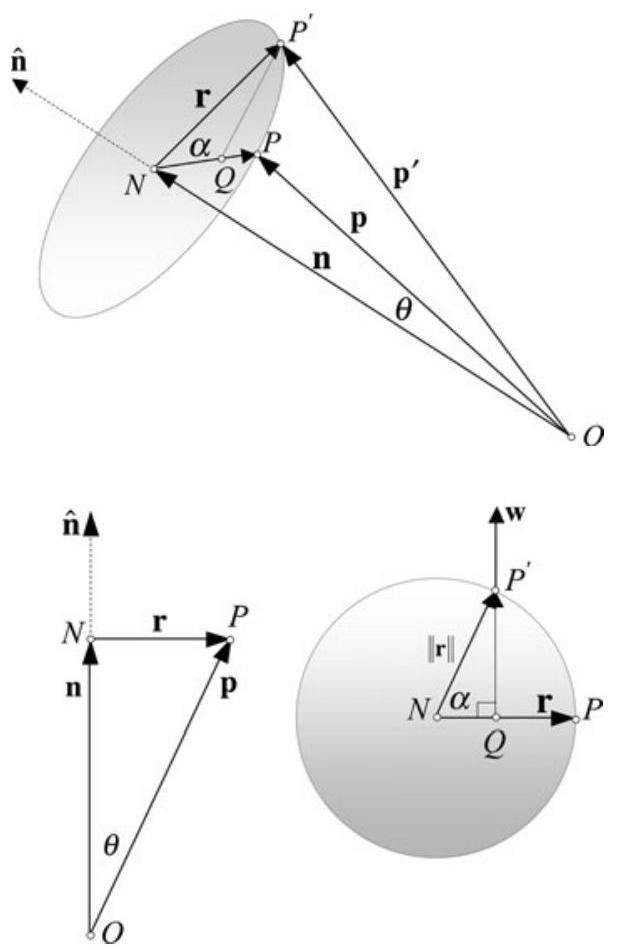
\includegraphics[max width=0.5\textwidth, center]{2023_01_16_a848224efad29cd66460g-095}
    \caption[short]{围绕任意轴旋转一点的几何学视图}
\end{figure}
\begin{figure}[h!]
    \centering
    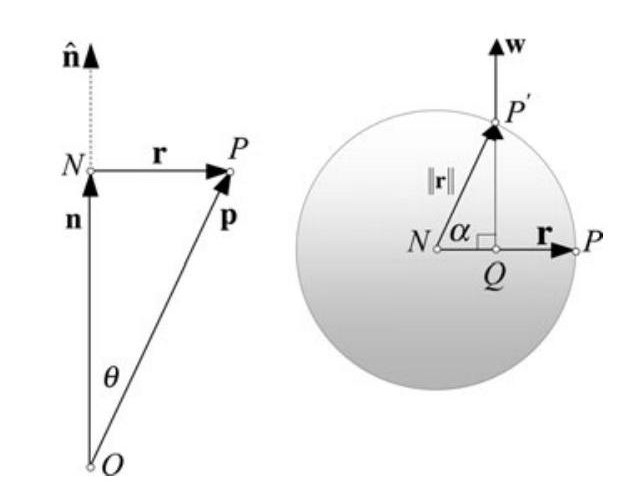
\includegraphics[max width=0.5\textwidth, center]{2023_01_16_a848224efad29cd66460g-095(1)}
    \caption[short]{绕任意轴旋转一点的几何学的横截面和平面视图}
\end{figure}

由图$6.7$和$6.8$:
$$
\mathbf{p}^{\prime}=\overrightarrow{O N}+\overrightarrow{N Q}+\overrightarrow{Q P^{\prime}}
$$

求 $\overrightarrow{O N}$
$$
|\mathbf{n}|=|\mathbf{p}| \cos \theta=\hat{\mathbf{n}} \cdot \mathbf{p}
$$

因此,
$$
\overrightarrow{O N}=\mathbf{n}=\hat{\mathbf{n}}(\hat{\mathbf{n}} \cdot \mathbf{p})
$$

求$\overrightarrow{N Q}$ :
$$
\overrightarrow{N Q}=\frac{N Q}{N P} \mathbf{r}=\frac{N Q}{N P^{\prime}} \mathbf{r}=\cos \alpha \mathbf{r}
$$

但
$$
\mathbf{p}=\mathbf{n}+\mathbf{r}=\hat{\mathbf{n}}(\hat{\mathbf{n}} \cdot \mathbf{p})+\mathbf{r}
$$

因此,
$$
\mathbf{r}=\mathbf{p}-\hat{\mathbf{n}}(\hat{\mathbf{n}} \cdot \mathbf{p})
$$

且
$$
\overrightarrow{N Q}=[\mathbf{p}-\hat{\mathbf{n}}(\hat{\mathbf{n}} \cdot \mathbf{p})] \cos \alpha
$$

求 $\overrightarrow{Q P^{\prime}}$ :

令
$$
\hat{\mathbf{n}} \times \mathbf{p}=\mathbf{w}
$$

其中
$$
|\mathbf{w}|=|\hat{\mathbf{n}}| \cdot|\mathbf{p}| \sin \theta=|\mathbf{p}| \sin \theta
$$

但
$$
|\mathbf{r}|=|\mathbf{p}| \sin \theta
$$

因此,
$$
|\mathbf{w}|=|\mathbf{r}| .
$$

现在
$$
\frac{Q P^{\prime}}{N P^{\prime}}=\frac{Q P^{\prime}}{|\mathbf{r}|}=\frac{Q P^{\prime}}{|\mathbf{w}|}=\sin \alpha
$$

因此,
$$
\overrightarrow{Q P^{\prime}}=\mathbf{w} \sin \alpha=(\hat{\mathbf{n}} \times \mathbf{p}) \sin \alpha
$$

接下来
$$
\mathbf{p}^{\prime}=\hat{\mathbf{n}}(\hat{\mathbf{n}} \cdot \mathbf{p})+(\mathbf{p}-\hat{\mathbf{n}}(\hat{\mathbf{n}} \cdot \mathbf{p})) \cos \alpha+(\hat{\mathbf{n}} \times \mathbf{p}) \sin \alpha
$$

且
$$
\mathbf{p}^{\prime}=\mathbf{p} \cos \alpha+\hat{\mathbf{n}}(\hat{\mathbf{n}} \cdot \mathbf{p})(1-\cos \alpha)+(\hat{\mathbf{n}} \times \mathbf{p}) \sin \alpha .
$$

令
$$
K=1-\cos \alpha
$$

\begin{figure}
    \centering
    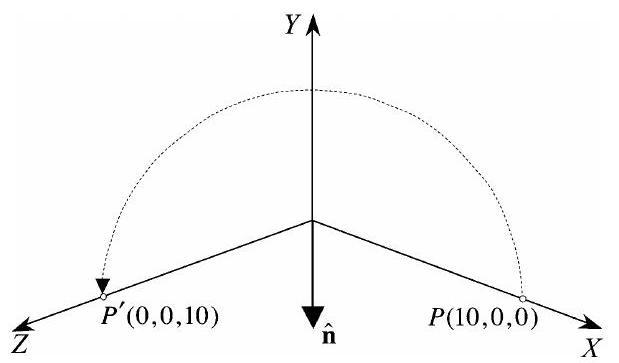
\includegraphics[max width=0.6\textwidth]{2023_01_16_a848224efad29cd66460g-097}
    \caption[short]{将点$P$从$180^{\circ}$旋转到$P^{\prime}$}
\end{figure}

接下来
$$
\mathbf{p}^{\prime}=\mathbf{p} \cos \alpha+\hat{\mathbf{n}}(\hat{\mathbf{n}} \cdot \mathbf{p}) K+(\hat{\mathbf{n}} \times \mathbf{p}) \sin \alpha
$$

且
$$
\begin{aligned}
\mathbf{p}^{\prime}= & \left(x_{p} \mathbf{i}+y_{p} \mathbf{j}+z_{p} \mathbf{k}\right) \cos \alpha+(a \mathbf{i}+b \mathbf{j}+c \mathbf{k})\left(a x_{p}+b y_{p}+c z_{p}\right) K \\
& +\left[\left(b z_{p}-c y_{p}\right) \mathbf{i}+\left(c x_{p}-a z_{p}\right) \mathbf{j}+\left(a y_{p}-b x_{p}\right) \mathbf{k}\right] \sin \alpha \\
\mathbf{p}^{\prime}= & {\left[x_{p} \cos \alpha+a\left(a x_{p}+b y_{p}+c z_{p}\right) K+\left(b z_{p}-c y_{p}\right) \sin \alpha\right] \mathbf{i} } \\
& +\left[y_{p} \cos \alpha+b\left(a x_{p}+b y_{p}+c z_{p}\right) K+\left(c x_{p}-a z_{p}\right) \sin \alpha\right] \mathbf{j} \\
& +\left[z_{p} \cos \alpha+c\left(a x_{p}+b y_{p}+c z_{p}\right) K+\left(a y_{p}-b x_{p}\right) \sin \alpha\right] \mathbf{k} \\
\mathbf{p}^{\prime}= & {\left[x_{p}\left(a^{2} K+\cos \alpha\right)+y_{p}(a b K-c \sin \alpha)+z_{p}(a c K+b \sin \alpha)\right] \mathbf{i} } \\
& +\left[x_{p}(a b K+c \sin \alpha)+y_{p}\left(b^{2} K+\cos \alpha\right)+z_{p}(b c K-a \sin \alpha)\right] \mathbf{j} \\
& +\left[x_{p}(a c K-b \sin \alpha)+y_{p}(b c K+a \sin \alpha)+z_{p}\left(c^{2} K+\cos \alpha\right)\right] \mathbf{k}
\end{aligned}
$$

它将解包到转换中:
$$
\left[\begin{array}{c}
x_{p}^{\prime} \\
y_{p}^{\prime} \\
z_{p}^{\prime}
\end{array}\right]=\left[\begin{array}{ccc}
a^{2} K+\cos \alpha & a b K-c \sin \alpha & a c K+b \sin \alpha \\
a b K+c \sin \alpha & b^{2} K+\cos \alpha & b c K-a \sin \alpha \\
a c K-b \sin \alpha & b c K+a \sin \alpha & c^{2} K+\cos \alpha
\end{array}\right]\left[\begin{array}{c}
x_{p} \\
y_{p} \\
z_{p}
\end{array}\right]
$$

其中
$$
K=1-\cos \alpha
$$

和用矩阵导出的变换是一样的。

让我们用一个容易验证的简单示例来测试转换。如果我们围绕$\hat{\mathbf{n}}=(1 / \sqrt{2}) \mathbf{i}+(1 / \sqrt{2}) \mathbf{k}$定义的轴旋转点$P(10,0,0), 180^{\circ}$,它应该被旋转到$P^{\prime}(0,0,10)$,如图6.9所示。因此,
$$
\begin{gathered}
\alpha=180^{\circ}, \quad \cos \alpha=-1, \quad \sin \alpha=0, \quad K=2, \\
a=\frac{1}{\sqrt{2}}, \quad b=0, \quad c=\frac{1}{\sqrt{2}}
\end{gathered}
$$

且
$$
\left[\begin{array}{c}
0 \\
0 \\
10
\end{array}\right]=\left[\begin{array}{ccc}
0 & 0 & 1 \\
0 & -1 & 0 \\
1 & 0 & 0
\end{array}\right]\left[\begin{array}{c}
10 \\
0 \\
0
\end{array}\right]
$$

这证实了我们的预测。

\section{总结}
在本章中,我们回顾了围绕三个笛卡尔轴之一旋转一个点的矩阵旋转变换。通过使用齐次坐标,可以将平移变换积分到围绕平行于一个笛卡尔轴的偏移轴旋转点。

复合旋转是通过组合表示围绕三个连续轴的单个旋转的矩阵来创建的。这样的旋转被称为欧拉旋转,有12种组合这些矩阵的方法。不幸的是,这种转换的问题之一是它们会受到万向节锁定的影响,在某些角度组合下会损失一个自由度。另一个问题是,虽然复合变换被广泛用于在世界空间中定位物体,但很难预测点在空间中如何移动。

最后,利用矩阵和向量建立了一个使一个点绕任意轴旋转的变换。

\subsection{变换总结}
\textbf{平移一个点}
$$
\mathbf{T}_{t_{x}, t_{y}, t_{z}}=\left[\begin{array}{cccc}
1 & 0 & 0 & t_{x} \\
0 & 1 & 0 & t_{y} \\
0 & 0 & 1 & t_{z} \\
0 & 0 & 0 & 1
\end{array}\right]
$$

\textbf{围绕$x-, y-, z$-轴旋转一个点}
$$
\begin{aligned}
\mathbf{R}_{\beta, x}= & {\left[\begin{array}{ccc}
1 & 0 & 0 \\
0 & \cos \beta & -\sin \beta \\
0 & \sin \beta & \cos \beta
\end{array}\right] } \\
\mathbf{R}_{\beta, y}= & {\left[\begin{array}{ccc}
\cos \beta & 0 & \sin \beta \\
0 & 1 & 0 \\
-\sin \beta & 0 & \cos \beta
\end{array}\right] } \\
\mathbf{R}_{\beta, z}= & {\left[\begin{array}{ccc}
\cos \beta & -\sin \beta & 0 \\
\sin \beta & \cos \beta & 0 \\
0 & 0 & 1
\end{array}\right] }
\end{aligned}
$$

\textbf{围绕偏移$x-, y-, z$-坐标轴旋转一个点}
$$
\begin{aligned}
\mathbf{R}_{\beta, x,\left(0, t_{y}, t_{z}\right)} & =\left[\begin{array}{cccc}
1 & 0 & 0 & 0 \\
0 & \cos \beta & -\sin \beta & t_{y}(1-\cos \beta)+t_{z} \sin \beta \\
0 & \sin \beta & \cos \beta & t_{z}(1-\cos \beta)-t_{y} \sin \beta \\
0 & 0 & 0 & 1
\end{array}\right] \\
\mathbf{R}_{\beta, y,\left(t_{x}, 0, t_{z}\right)} & =\left[\begin{array}{cccc}
\cos \beta & 0 & \sin \beta & t_{x}(1-\cos \beta)-t_{z} \sin \beta \\
0 & 1 & 0 & 0 \\
-\sin \beta & 0 & \cos \beta & t_{z}(1-\cos \beta)+t_{x} \sin \beta \\
0 & 0 & 0 & 1
\end{array}\right] \\
\mathbf{R}_{\beta, z,\left(t_{x}, t_{y}, 0\right)} & =\left[\begin{array}{cccc}
\cos \beta & -\sin \beta & 0 & t_{x}(1-\cos \beta)+t_{y} \sin \beta \\
\sin \beta & \cos \beta & 0 & t_{y}(1-\cos \beta)-t_{x} \sin \beta \\
0 & 0 & 1 & 0 \\
0 & 0 & 0 & 1
\end{array}\right]
\end{aligned}
$$

\textbf{绕任意轴旋转一点}
$$
\begin{aligned}
\mathbf{R}_{\alpha, \hat{\mathbf{n}}} & =\left[\begin{array}{ccc}
a^{2} K+\cos \alpha & a b K-c \sin \alpha & a c K+b \sin \alpha \\
a b K+c \sin \alpha & b^{2} K+\cos \alpha & b c K-a \sin \alpha \\
a c K-b \sin \alpha & b c K+a \sin \alpha & c^{2} K+\cos \alpha
\end{array}\right] \\
K & =1-\cos \alpha \\
\hat{\mathbf{n}} & =a \mathbf{i}+b \mathbf{j}+c \mathbf{k} .
\end{aligned}
$$

\section{样例}
下面是一些进一步使用上述思想的示例。在某些情况下,包括测试来确认结果。

\begin{example}
    建立一个旋转变换,使一个点围绕偏移于$y$-轴的轴旋转。
    
    设偏移轴与点$\left(t_{x}, 0, t_{z}\right)$相交。因此,这个旋转的齐次变换是
    $$
    \left[\begin{array}{c}
    x^{\prime} \\
    y^{\prime} \\
    z^{\prime} \\
    1
    \end{array}\right]=\mathbf{T}_{t_{x}, 0, t_{z}} \mathbf{R}_{\beta, y} \mathbf{T}_{-t_{x}, 0,-t_{z}}\left[\begin{array}{c}
    x \\
    y \\
    z \\
    1
    \end{array}\right]
    $$
    
    其中
    $$
    \begin{aligned}
    & \mathbf{T}_{-t_{x}, 0,-t_{z}} && \text { 创建临时原点 } \\
    & \mathbf{R}_{\beta, y} && \text { 围绕临时的 } y \text {轴旋转 }\beta \text{角度} \\
    & \mathbf{T}_{t_{x}, 0, t_{z}} && \text { 返回原来的坐标原点位置 }
    \end{aligned}
    $$
    
    且
    $$
    \begin{aligned}
    \mathbf{T}_{t_{x}, 0, t_{z}} & =\left[\begin{array}{llll}
    1 & 0 & 0 & t_{x} \\
    0 & 1 & 0 & 0 \\
    0 & 0 & 1 & t_{z} \\
    0 & 0 & 0 & 1
    \end{array}\right] \\
    \mathbf{T}_{-t_{x}, 0,-t_{z}} & =\left[\begin{array}{cccc}
    1 & 0 & 0 & -t_{x} \\
    0 & 1 & 0 & 0 \\
    0 & 0 & 1 & -t_{z} \\
    0 & 0 & 0 & 1
    \end{array}\right] \\
    \mathbf{R}_{\beta, y} & =\left[\begin{array}{cccc}
    \cos \beta & 0 & \sin \beta & 0 \\
    0 & 1 & 0 & 0 \\
    -\sin \beta & 0 & \cos \beta & 0 \\
    0 & 0 & 0 & 1
    \end{array}\right] .
    \end{aligned}
    $$
    
    因此,
    $$
    \begin{aligned}
    & \mathbf{T}_{t_{x}, 0, t_{z}} \mathbf{R}_{\beta, y} \mathbf{T}_{-t_{x}, 0,-t_{z}} \\
    &= {\left[\begin{array}{cccc}
    1 & 0 & 0 & t_{x} \\
    0 & 1 & 0 & 0 \\
    0 & 0 & 1 & t_{z} \\
    0 & 0 & 0 & 1
    \end{array}\right]\left[\begin{array}{cccc}
    \cos \beta & 0 & \sin \beta & 0 \\
    0 & 1 & 0 & 0 \\
    -\sin \beta & 0 & \cos \beta & 0 \\
    0 & 0 & 0 & 1
    \end{array}\right]\left[\begin{array}{cccc}
    1 & 0 & 0 & -t_{x} \\
    0 & 1 & 0 & 0 \\
    0 & 0 & 1 & -t_{z} \\
    0 & 0 & 0 & 1
    \end{array}\right] } \\
    &= {\left[\begin{array}{cccc}
    1 & 0 & 0 & t_{x} \\
    0 & 1 & 0 & 0 \\
    0 & 0 & 1 & t_{z} \\
    0 & 0 & 0 & 1
    \end{array}\right]\left[\begin{array}{cccc}
    \cos \beta & 0 & \sin \beta & -t_{x} \cos \beta-t_{z} \sin \beta \\
    0 & 1 & 0 & 0 \\
    -\sin \beta & 0 & \cos \beta & t_{x} \sin \beta-t_{z} \cos \beta \\
    0 & 0 & 0 & 1
    \end{array}\right] } \\
    &= {\left[\begin{array}{ccccc}
    \cos \beta & 0 & \sin \beta & t_{x}(1-\cos \beta)-t_{z} \sin \beta \\
    0 & 1 & 0 & 0 \\
    -\sin \beta & 0 & \cos \beta & t_{z}(1-\cos \beta)+t_{x} \sin \beta \\
    0 & 0 & 0 & 1
    \end{array}\right] }
    \end{aligned}
    $$
\end{example}

\begin{example}
    计算$\mathbf{R}_{\gamma, x} \mathbf{R}_{\beta, y} \mathbf{R}_{\alpha, x}$的旋转变换,看看当$\alpha=\beta=\gamma=90^{\circ}$时,它是否会出现万向锁。旋转轴和角度是多少?
    
    使用符号$c_{\beta}=\cos \beta$和$s_{\beta}=\sin \beta$,复合转换为
    $$
    \begin{aligned}
    \mathbf{R}_{\gamma, x} \mathbf{R}_{\beta, y} \mathbf{R}_{\alpha, x} & =\left[\begin{array}{ccc}
    1 & 0 & 0 \\
    0 & c_{\gamma} & -s_{\gamma} \\
    0 & s_{\gamma} & c_{\gamma}
    \end{array}\right]\left[\begin{array}{ccc}
    c_{\beta} & 0 & s_{\beta} \\
    0 & 1 & 0 \\
    -s_{\beta} & 0 & c_{\beta}
    \end{array}\right]\left[\begin{array}{ccc}
    1 & 0 & 0 \\
    0 & c_{\alpha} & -s_{\alpha} \\
    0 & s_{\alpha} & c_{\alpha}
    \end{array}\right] \\
    & =\left[\begin{array}{ccc}
    c_{\beta} & s_{\beta} s_{\alpha} & s_{\beta} c_{\alpha} \\
    s_{\gamma} s_{\beta} & \left(c_{\gamma} c_{\alpha}-s_{\gamma} c_{\beta} s_{\alpha}\right) & \left(-c_{\gamma} s_{\alpha}-s_{\gamma} c_{\beta} c_{\alpha}\right) \\
    -c_{\gamma} s_{\beta} & \left(s_{\gamma} c_{\alpha}+c_{\gamma} c_{\beta} s_{\alpha}\right) & \left(-s_{\gamma} s_{\alpha}+c_{\gamma} c_{\beta} c_{\alpha}\right)
    \end{array}\right] \\
    \mathbf{R}_{90^{\circ}, x} \mathbf{R}_{90^{\circ}, y} \mathbf{R}_{90^{\circ}, x} & =\left[\begin{array}{ccc}
    0 & 1 & 0 \\
    1 & 0 & 0 \\
    0 & 0 & -1
    \end{array}\right] .
    \end{aligned}
    $$
    
    图$6.10$显示了立方体在旋转的每个阶段,很明显,万向节锁不存在,因为立方体通过其每个正交轴旋转。旋转轴是通过顶点0和6,即$\left[\begin{array}{lll}1 & 1 & 0\end{array}\right]^{\mathrm{T}}$,旋转角度为$180^{\circ}$。
    
    \begin{figure}[h!]
        \centering
        \subfigure[caption]{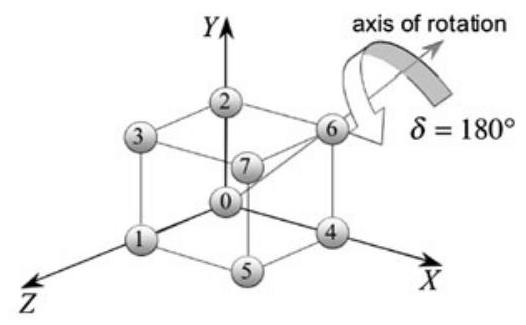
\includegraphics[max width=0.35\textwidth]{2023_01_16_a848224efad29cd66460g-101}}
        \subfigure[caption]{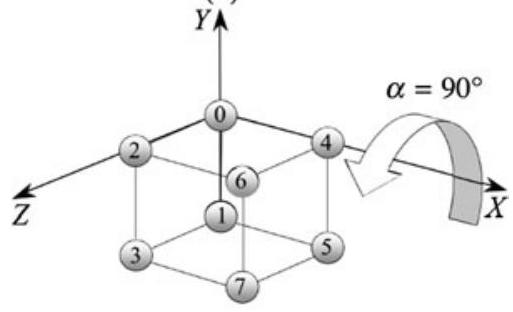
\includegraphics[max width=0.35\textwidth]{2023_01_16_a848224efad29cd66460g-101(2)}}\\
        \subfigure[caption]{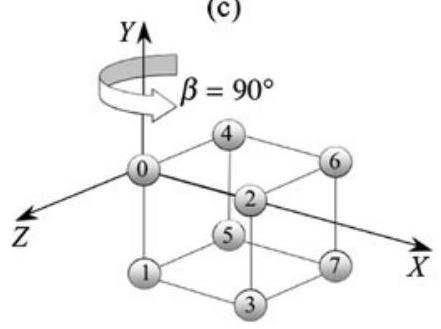
\includegraphics[max width=0.35\textwidth]{2023_01_16_a848224efad29cd66460g-101(1)}}
        \subfigure[caption]{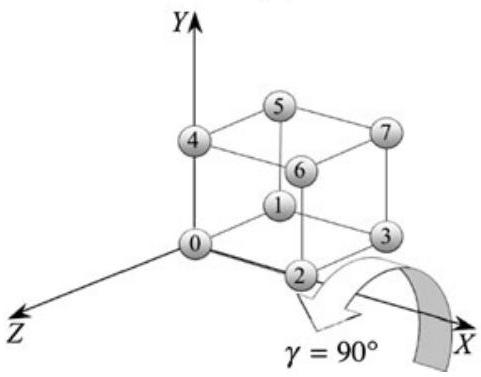
\includegraphics[max width=0.35\textwidth]{2023_01_16_a848224efad29cd66460g-101(3)}}
        \caption[short]{单元立方体在三次旋转之前和过程中的四个视图$\mathbf{R}_{90^{\circ}, x} \mathbf{R}_{90^{\circ}, y} \mathbf{R}_{90^{\circ}, x}$}
    \end{figure}
\end{example}

\begin{example}
    证明任意轴上旋转点的旋转矩阵适用于三个笛卡尔轴。
    
    从这个矩阵开始:
    
    $$
    \begin{aligned}
    \mathbf{R}_{\alpha, \hat{\mathbf{n}}} & =\left[\begin{array}{ccc}
    a^{2} K+\cos \alpha & a b K-c \sin \alpha & a c K+b \sin \alpha \\
    a b K+c \sin \alpha & b^{2} K+\cos \alpha & b c K-a \sin \alpha \\
    a c K-b \sin \alpha & b c K+a \sin \alpha & c^{2} K+\cos \alpha
    \end{array}\right] \\
    K & =1-\cos \alpha \\
    \hat{\mathbf{n}} & =a \mathbf{i}+b \mathbf{j}+c \mathbf{k} .
    \end{aligned}
    $$
    
    绕$x$轴旋转:
    $$
    \hat{\mathbf{n}}=a \mathbf{i}
    $$
    
    因此,$a=1$, $b=c=0$:
    $$
    \mathbf{R}_{\alpha, x}=\left[\begin{array}{ccc}
    1 & 0 & 0 \\
    0 & \cos \alpha & -\sin \alpha \\
    0 & \sin \alpha & \cos \alpha
    \end{array}\right] .
    $$
    
    绕$y$轴旋转:
    $$
    \hat{\mathbf{n}}=b \mathbf{j}
    $$
    
    因此, $b=1$, $a=c=0$ :
    $$
    \mathbf{R}_{\alpha, y}=\left[\begin{array}{ccc}
    \cos \alpha & 0 & \sin \alpha \\
    0 & 1 & 0 \\
    -\sin \alpha & 0 & \cos \alpha
    \end{array}\right]
    $$
    
    绕$z$轴旋转:
    $$
    \hat{\mathbf{n}}=c \mathbf{k}
    $$
    
    因此,$c=1$,$a=b=0$ :
    
    $$
    \mathbf{R}_{\alpha, z}=\left[\begin{array}{ccc}
    \cos \alpha & -\sin \alpha & 0 \\
    \sin \alpha & \cos \alpha & 0 \\
    0 & 0 & 1
    \end{array}\right]
    $$
    
    这是正确的。
\end{example}

\begin{example}
    计算旋转变换,使一个点围绕一个与$\left[\begin{array}{lll}1 & 1 & 1\end{array}\right]^{\mathrm {T}}$对齐的轴旋转$180^{\circ}$。举个例子,通过这个变换将一个点旋转两次将其返回到它原来的位置。
    
    从矩阵开始:
    $$
    \begin{aligned}
    \mathbf{R}_{\alpha, \hat{\mathbf{n}}} & =\left[\begin{array}{ccc}
    a^{2} K+\cos \alpha & a b K-c \sin \alpha & a c K+b \sin \alpha \\
    a b K+c \sin \alpha & b^{2} K+\cos \alpha & b c K-a \sin \alpha \\
    a c K-b \sin \alpha & b c K+a \sin \alpha & c^{2} K+\cos \alpha
    \end{array}\right] \\
    K & =1-\cos \alpha \\
    \hat{\mathbf{n}} & =a \mathbf{i}+b \mathbf{j}+c \mathbf{k} .
    \end{aligned}
    $$
    
    因此,给出 $\mathbf{n}=\mathbf{i}+\mathbf{j}+\mathbf{k}$
    
    $$
    \hat{\mathbf{n}}=\frac{1}{\sqrt{3}} \mathbf{i}+\frac{1}{\sqrt{3}} \mathbf{j}+\frac{1}{\sqrt{3}} \mathbf{k}
    $$
    
    且
    
    $$
    a=b=c=\frac{1}{\sqrt{3}} \text {. }
    $$
    
    给出 $\alpha=180^{\circ}, \cos \alpha=-1, \sin \alpha=0$ 且 $K=2$, 矩阵就变成了:
    $$
    \mathbf{R}_{180^{\circ}, \hat{\mathbf{n}}}=\left[\begin{array}{ccc}
    -1 / 3 & 2 / 3 & 2 / 3 \\
    2 / 3 & -1 / 3 & 2 / 3 \\
    2 / 3 & 2 / 3 & -1 / 3
    \end{array}\right] \text {. }
    $$
    
    这个矩阵与自身相乘必然得到单位矩阵:
    $$
    \begin{aligned}
    \mathbf{R}_{180^{\circ}, \hat{\mathbf{n}}} \mathbf{R}_{180^{\circ}, \hat{\mathbf{n}}} & =\left[\begin{array}{ccc}
    -1 / 3 & 2 / 3 & 2 / 3 \\
    2 / 3 & -1 / 3 & 2 / 3 \\
    2 / 3 & 2 / 3 & -1 / 3
    \end{array}\right]\left[\begin{array}{ccc}
    -1 / 3 & 2 / 3 & 2 / 3 \\
    2 / 3 & -1 / 3 & 2 / 3 \\
    2 / 3 & 2 / 3 & -1 / 3
    \end{array}\right] \\
    & =\left[\begin{array}{ccc}
    1 & 0 & 0 \\
    0 & 1 & 0 \\
    0 & 0 & 1
    \end{array}\right]
    \end{aligned}
    $$
    
    这证实了任意点经过这个旋转矩阵旋转两次后都回到了原点。
\end{example}
